\begin{remark}
  The size of any matching \(M\) in \(G\) is at most \(n/2\). That is,
  \[ |M| \leq |V(G)| \]
\end{remark}

\section{Matching in Bipartite Graph}

\begin{definition}[Neighborhood]
  For a vertex \(v \in V(G)\), the \textit{neighborhood} of \(v\), denoted
  \(N(v)\) is the set of vertices that are adjacent to \(v\).
  Similarly, we also denote \(N(S)\) for some non-empty set \(S\) of
  vertices to be the union of all neighborhood of vertices in \(S\).
\end{definition}

\begin{definition}[Alternating Path]
  An \textit{alternating path} is a path that alternates between matching and
  non-matching edges.
\end{definition}

\begin{definition}[Augmenting Path]
  An \textit{augmenting path} is an alternating path that starts and ends on
  unmatchated vertices.
\end{definition}

The matching problem in bipartite setting is often called the \textit{marriage
problem}. That is, if there are a finite set of girls, each of whom knows
several boys, under what conditions can all the girls marry the boys in such a
way that each girl marries a boy she knows? The sufficient condition is claimed
and proven in Hall's Marriage Theorem.

\begin{theorem}[Hall's Marriage Theorem]
  A bipartite graph \(G\) contains a matching of \(A\) if and only if \(|N(S)|
  \geq |S|\) for every \(S \subseteq A\) where \(A\) refers to one of the two
  sets of vertices in the graph. The condition present in the theorem is also 
  known as the \textit{marriage condition}.
\end{theorem}

\begin{proof}
  First, we will show the forward direction: If \(G\) contains a matching of
  \(A\), then \(|N(S)| \geq |S|\) for every \(S \subseteq A\). Assume that there
  is \(S \subseteq A\) such that \(|N(S)| < |S|\). Then, it is clear that there
  is no matching for the set \(S\) since there isn't enough vertices in \(N(S)\)
  for vertices in \(S\) to match with.

  Now, we will show the inverse direction: If the marriage condition satisfies,
  then \(G\) contains a matching. Consider a graph \(G\) where the marriage
  condition satisfies. Suppose that we already have an imperfect matching \(M\)
  in \(G\).
  \begin{enumerate}[label=\textit{Step \arabic*.}]
    \item Pick an unmatched vertex \(a_0\) in \(G\) and put
      it in a set \(\overline{A}\). 
    \item Randomly select a vertex \(b \in N(a_0)\) and put it in \(\overline{B}\).
    \item There are now two cases:
      \begin{itemize}
        \item If \(b\) is not part of the matching, then we are done. Then, we can
          find an augmenting path by backtracking from \(a_0 \to \cdots \to b\) to
          be another alternating path. 
        \item Otherwise, \(b\) is already part of \(M\). Suppose that \(b\) is
          already paired with \(a_i \in A\). Then, let \(\overline{A} = \{a_i\} \cup
          \overline{A}\) and repeat step 2. The algorithm will terminate when all
          vertices are matched.
      \end{itemize}
  \end{enumerate}
\end{proof}

\begin{remark}
  By the marriage condition, we can always find a vertex \(b \in B\) to include
  in \(\overline{B}\) in step 2.
\end{remark}

\begin{proof}[Alternate Inverse Direction Proof]
  % We will show this by induction on \(|A|\). Consider the base case when
  % \(|A| = 1\). Then, there is a matching of \(A\) by matching the vertex in
  % \(A\) to any vertex in \(B\).

  % Now, we will show the inductive case. Let \(|A| \geq 2\) and assume that 
  % the marriage condition implies that there is a matching of \(A\) when 
  % \(|A| = k\). We will now show that this holds when \(|A| = k+1\). There are
  % cases for us to consider: 
  % \begin{enumerate}[label=\textit{Case \arabic*.}]
  %   \item If \(|N(S)| \geq |S| + 1\) for every non-empty set \(S \subsetneq A\).
  %     Pick any edge \(e = (a, b) \in E(G)\) and consider the graph \(G' =
  %     G-(a,b)\). Then, every non-empty set \(S \subseteq A \setminus \{a\}\)
  %     satisfies \(|N_G(S)| \geq |N_G(S)| - 1 \geq |S|\). Thus, the marriage
  %     condition still satisfies and by induction, \(G'\) contains a matching of
  %     \(A \setminus \{a\}\). Together with the edge of \((a, b)\), this yields a
  %     matching of \(A\) in \(G\).
  %   \item Otherwise, there is \(A' \subsetneq A\) such that \(|N(A')| = |A'|\). 
  %     Then, \(G' = A' \cup N(A')\) contains a matching of \(A'\) by the
  %     induction hypothesis. On the otherhand, \(G-G'\) satisfies the marriage
  %     condition as well. This is because if \(S \subseteq A \setminus A'\)
  %     satisfies \(|N_{G-G'}(S)| < |S|\), we could have \(|N_G(S \cup A')| < |S
  %     \cup A'|\) which contradicts the inductive hypothesis. So again
  % \end{enumerate}
  [Requires rewrite]
\end{proof}

\begin{theorem}[The Marriage Theorem]
  In a collection of \(r\) women and \(r\) men, a total of \(r\) marriages 
  between acquainted couples is possible if and only if for each integer \(k\)
  when \(1 \leq k \leq r\), every subset of \(k\) women is collectively 
  acquainted with at least \(k\) men.
\end{theorem}

\begin{figure}[ht]
\begin{nexample}
  Explain why the graph below has no complete matching from \(V_1\) to \(V_2\).
  When does the marriage condition fail?

  \begin{center}
    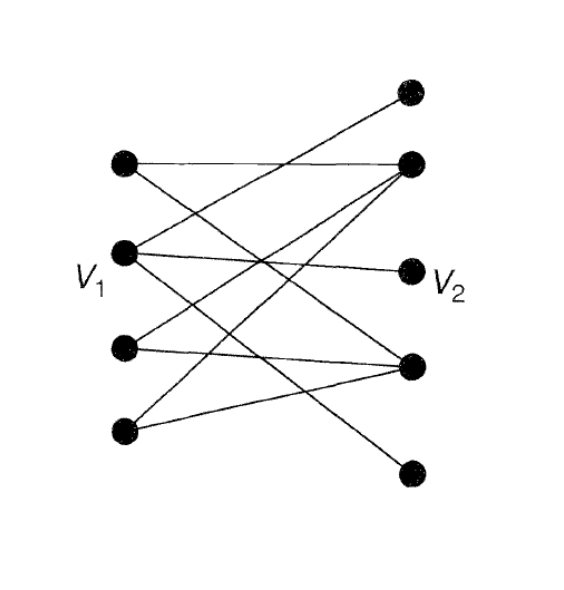
\includegraphics[width=0.4\textwidth]{figures/l07/marriage-fails.png}
  \end{center}

  Notice that when \(S = \{v_{1,1}, v_{1,3}, v_{1,4}\}\), then we have that 
  \[ |N(S)| = 2 > |S| = 3 \] 
  Hence, this fails the marriage condition.
\end{nexample}
\end{figure}
